Use of a typing element similar to IBM Selectric typewriter as shown in figure \ref{fig:IBM_Selectric_Globe_Wiki.jpg}. Viable for a printer, however the moving mechanism is too large to be embedded into a tablet-sized device. Hybrid addressable cell attempts to tackle the size issue.
\begin{figure}
\centering
    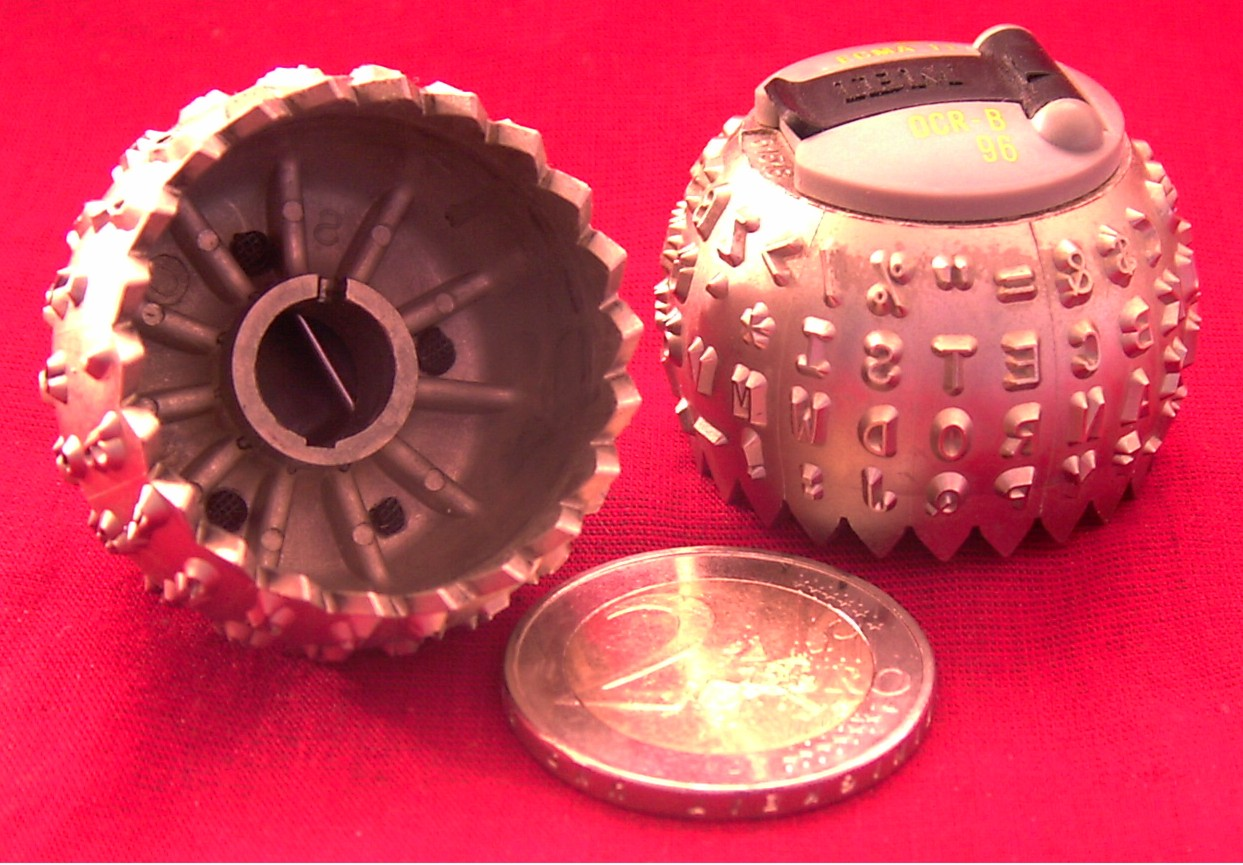
\includegraphics[height=5cm]{figures/IBM_Selectric_Globe_Wiki.jpg}
\caption[IBM Selectric typing element]{IBM Selectric typing element \cite{wiki:IBMSelectric}.}
\label{fig:IBM_Selectric_Globe_Wiki.jpg}
\end{figure}

An alternative that addresses the size is shown in figure \ref{fig:rotation.png}, wherein the characters fall partially into a slot, resulting in their depression on the surface. Each rotating disk is a saggital half of the braille cell, i.e. two disks form one braille cell. Roberts et al explore similar ideas \cite{roberts_492_2000}, and faced issues with component wear and the mechanism jamming.

\begin{figure}
\centering
    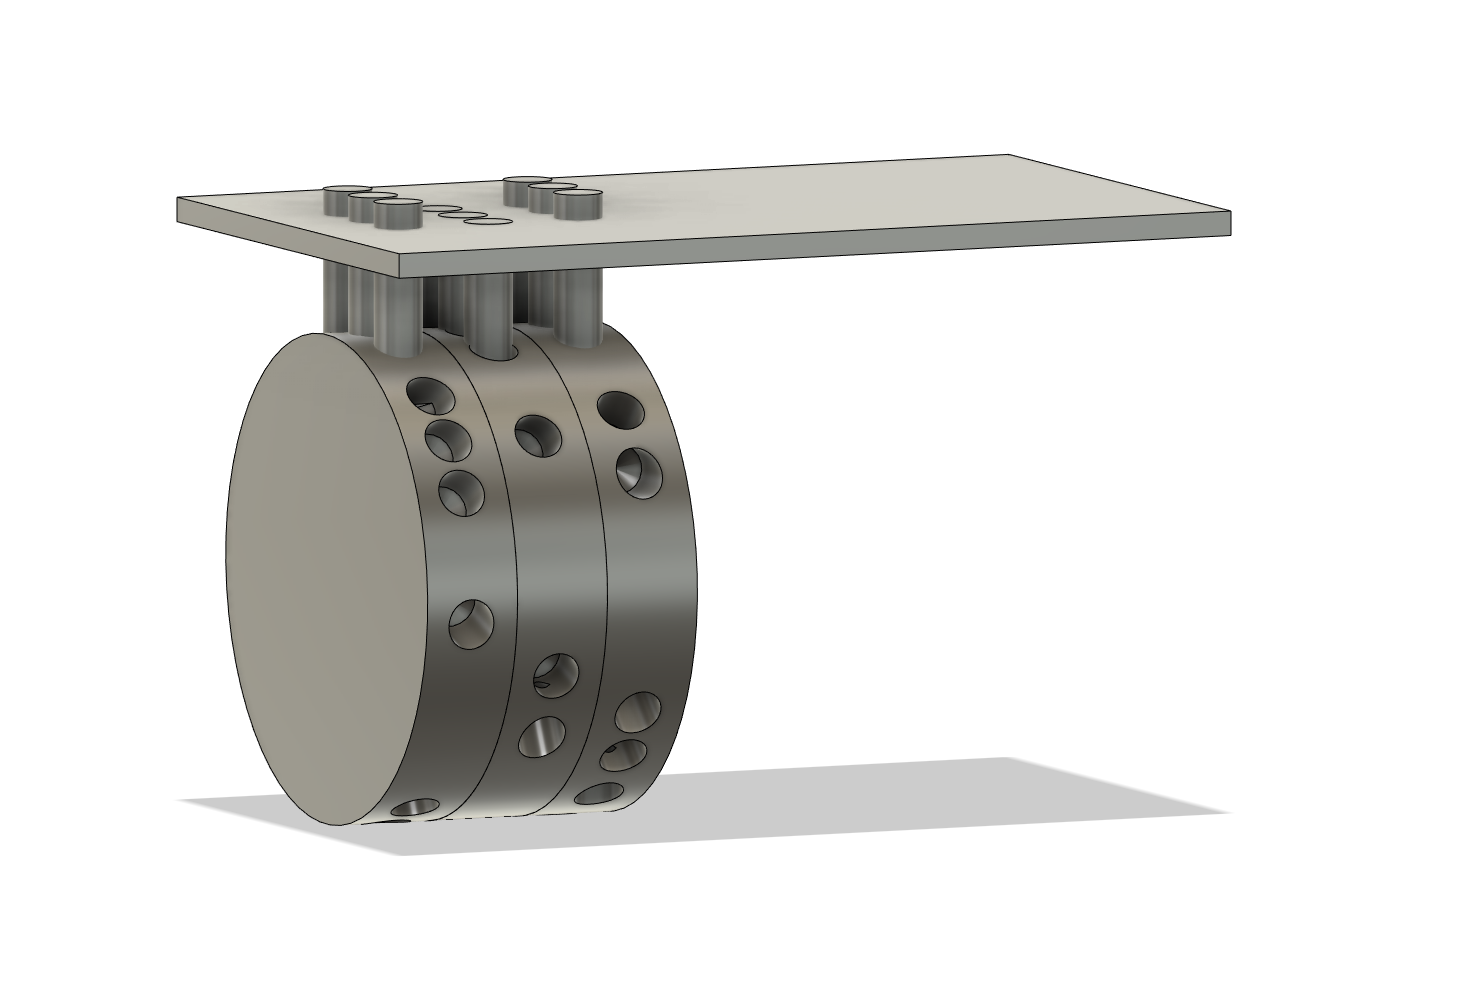
\includegraphics[width=0.6\textwidth]{figures/rotation.png}
\caption{Hybrid addressable cell. Holes on the disk define which pins are depressed on the surface.}
\label{fig:rotation.png}
\end{figure}